\documentclass[11pt]{article}
\usepackage[textwidth=18.0cm, textheight=23.0cm, top=2.0cm]{geometry}
\usepackage{pst-all}
\usepackage{amssymb}
\usepackage{tikz}
\usepackage{underscore}\begin{document}
\pagestyle{empty}


ClassName: \underline{\textbf{Class_07.2bp-11}}
\par
BinSize: \underline{\textbf{100 × 100}}
\par
ReduceSize: \underline{\textbf{100 × 100}}
\par
TypeNum: \underline{\textbf{39}}
\par
Num: \underline{\textbf{40}}
\par
OutS: \underline{\textbf{120000}}
\par
InS: \underline{\textbf{103150}}
\par
Rate: \underline{\textbf{0.860}}
\par
UB: \underline{\textbf{12}}
\par
LB0: \underline{\textbf{12}}
\par
LB: \underline{\textbf{12}}
\par
LBWithCut: \underline{\textbf{12}}
\par
NodeCut: \underline{\textbf{0}}
\par
ExtendedNodeCnt: \underline{\textbf{1}}
\par
GenNodeCnt: \underline{\textbf{1}}
\par
PrimalNode: \underline{\textbf{0}}
\par
ColumnCount: \underline{\textbf{12}}
\par
TotalCutCount: \underline{\textbf{0}}
\par
RootCutCount: \underline{\textbf{0}}
\par
LPSolverCnt: \underline{\textbf{1}}
\par
PricingSolverCnt: \underline{\textbf{0}}
\par
BranchAndBoundNum: \underline{\textbf{1}}
\par
isOpt: \underline{\textbf{true}}
\par
TimeOnInitSolution: \underline{\textbf{600.000 s}}
\par
TimeOnPrimal: \underline{\textbf{0.000 s}}
\par
TimeOnPricing: \underline{\textbf{0.000 s}}
\par
TimeOnRmp: \underline{\textbf{0.063 s}}
\par
TotalTime: \underline{\textbf{600.311 s}}
\par
\newpage


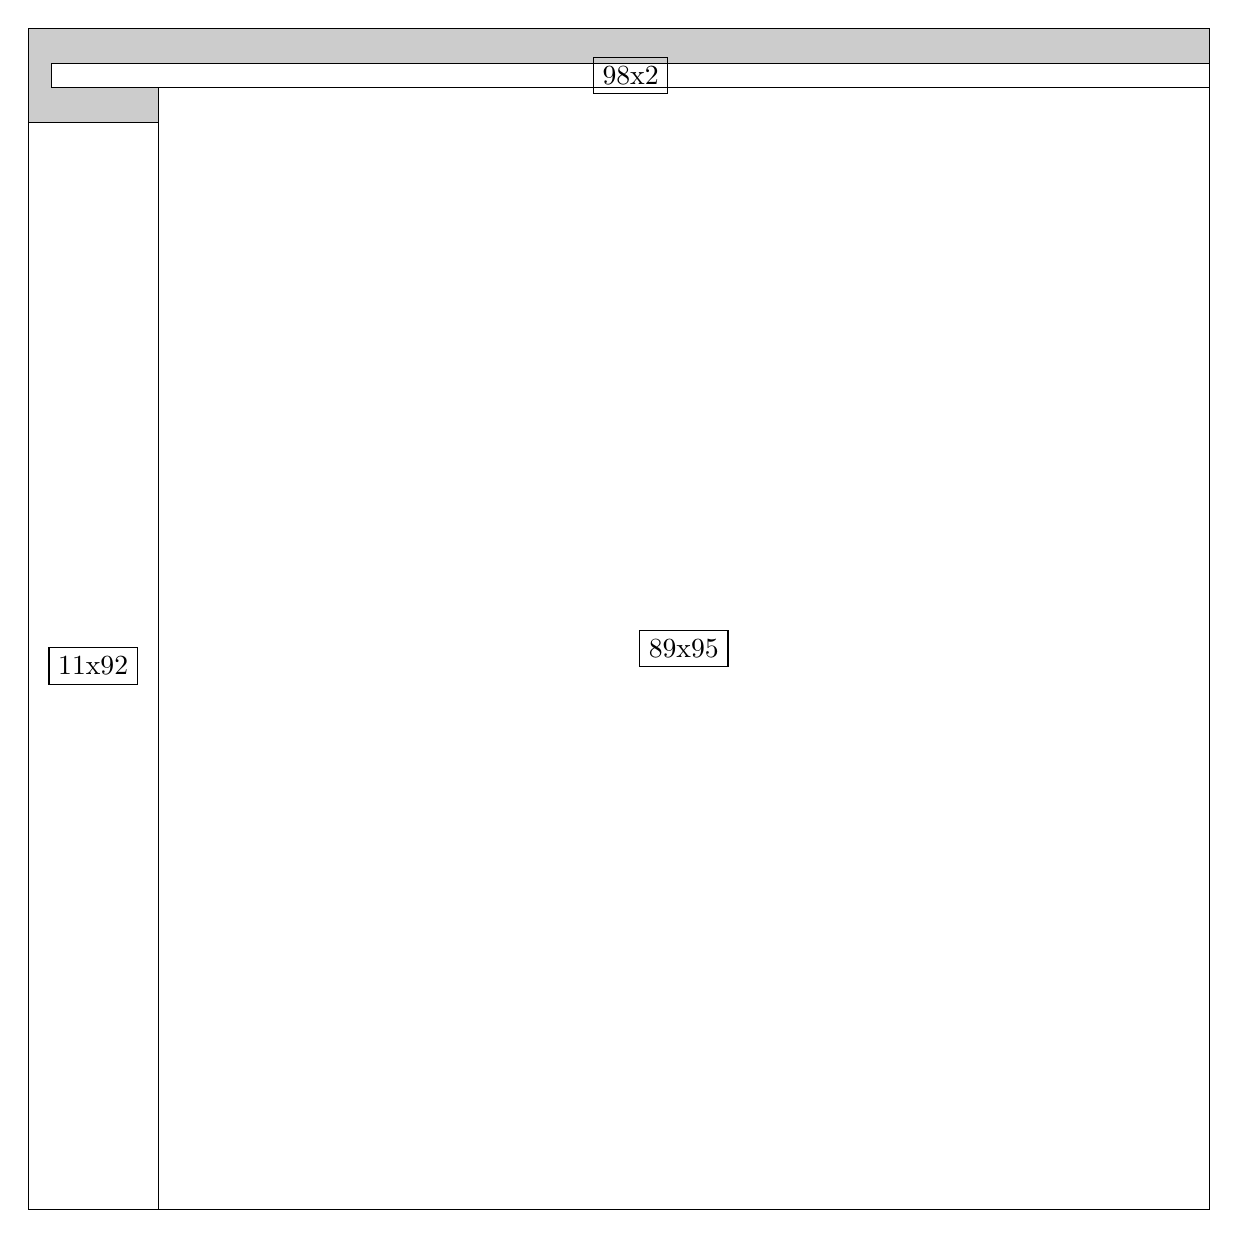
\begin{tikzpicture}[shorten >=1pt,scale=1.0,every node/.style={scale=1.0},->]
\tikzstyle{vertex}=[circle,fill=black!25,minimum size=14pt,inner sep=0pt]
\filldraw[fill=gray!40!white, draw=black] (0,0) rectangle (15.0,15.0);
\foreach \name/\x/\y/\w/\h in {89x95/1.65/0.0/13.35/14.25,11x92/0.0/0.0/1.65/13.799999999999999,98x2/0.3/14.25/14.7/0.3}
\filldraw[fill=white!40!white, draw=black] (\x,\y) rectangle node[draw] (\name) {\name} ++(\w,\h);
\end{tikzpicture}


w =89 , h =95 , x =11 , y =0 , v =8455
\par
w =11 , h =92 , x =0 , y =0 , v =1012
\par
w =98 , h =2 , x =2 , y =95 , v =196
\par
\newpage


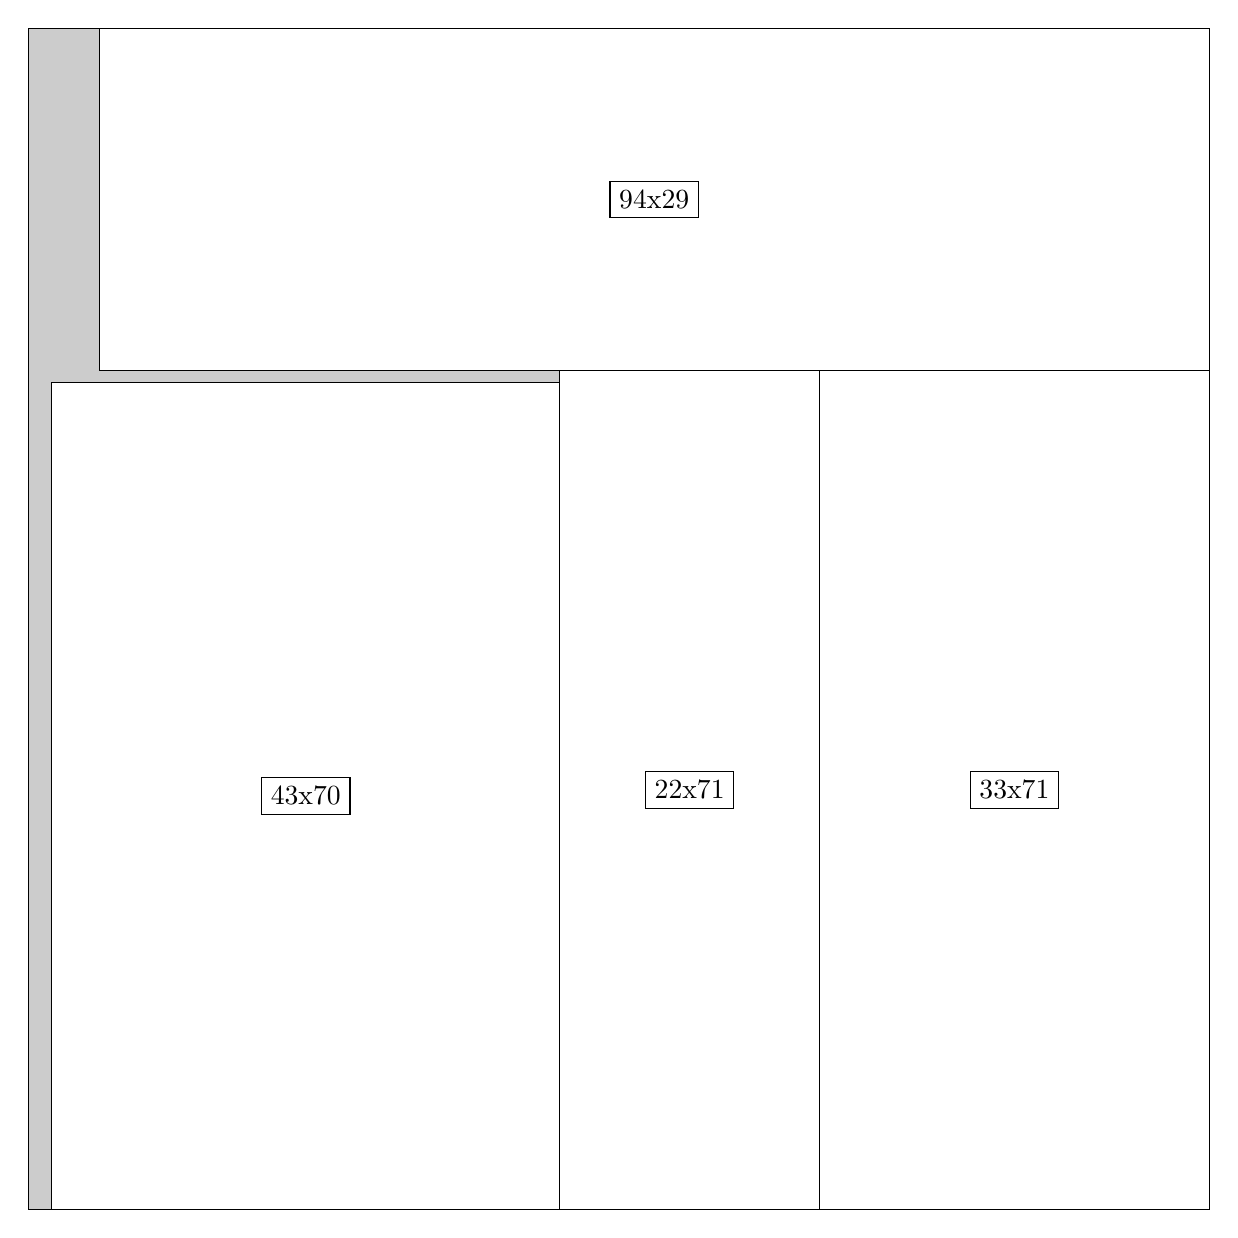
\begin{tikzpicture}[shorten >=1pt,scale=1.0,every node/.style={scale=1.0},->]
\tikzstyle{vertex}=[circle,fill=black!25,minimum size=14pt,inner sep=0pt]
\filldraw[fill=gray!40!white, draw=black] (0,0) rectangle (15.0,15.0);
\foreach \name/\x/\y/\w/\h in {33x71/10.049999999999999/0.0/4.95/10.65,22x71/6.75/0.0/3.3/10.65,43x70/0.3/0.0/6.45/10.5,94x29/0.8999999999999999/10.65/14.1/4.35}
\filldraw[fill=white!40!white, draw=black] (\x,\y) rectangle node[draw] (\name) {\name} ++(\w,\h);
\end{tikzpicture}


w =33 , h =71 , x =67 , y =0 , v =2343
\par
w =22 , h =71 , x =45 , y =0 , v =1562
\par
w =43 , h =70 , x =2 , y =0 , v =3010
\par
w =94 , h =29 , x =6 , y =71 , v =2726
\par
\newpage


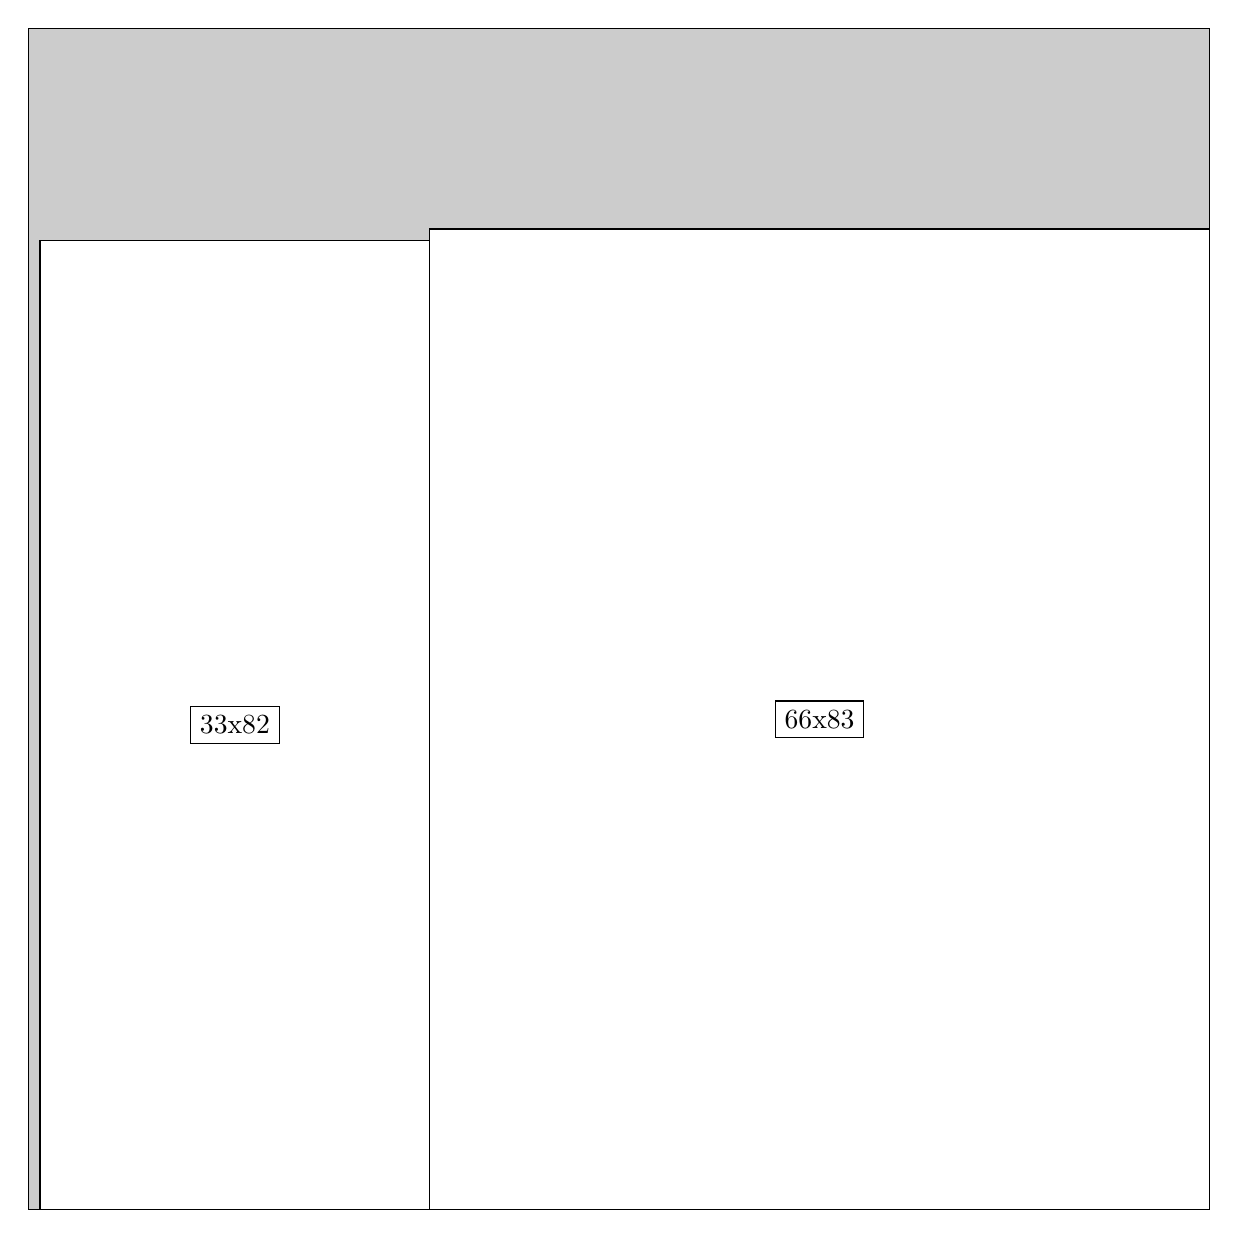
\begin{tikzpicture}[shorten >=1pt,scale=1.0,every node/.style={scale=1.0},->]
\tikzstyle{vertex}=[circle,fill=black!25,minimum size=14pt,inner sep=0pt]
\filldraw[fill=gray!40!white, draw=black] (0,0) rectangle (15.0,15.0);
\foreach \name/\x/\y/\w/\h in {66x83/5.1/0.0/9.9/12.45,33x82/0.15/0.0/4.95/12.299999999999999}
\filldraw[fill=white!40!white, draw=black] (\x,\y) rectangle node[draw] (\name) {\name} ++(\w,\h);
\end{tikzpicture}


w =66 , h =83 , x =34 , y =0 , v =5478
\par
w =33 , h =82 , x =1 , y =0 , v =2706
\par
\newpage


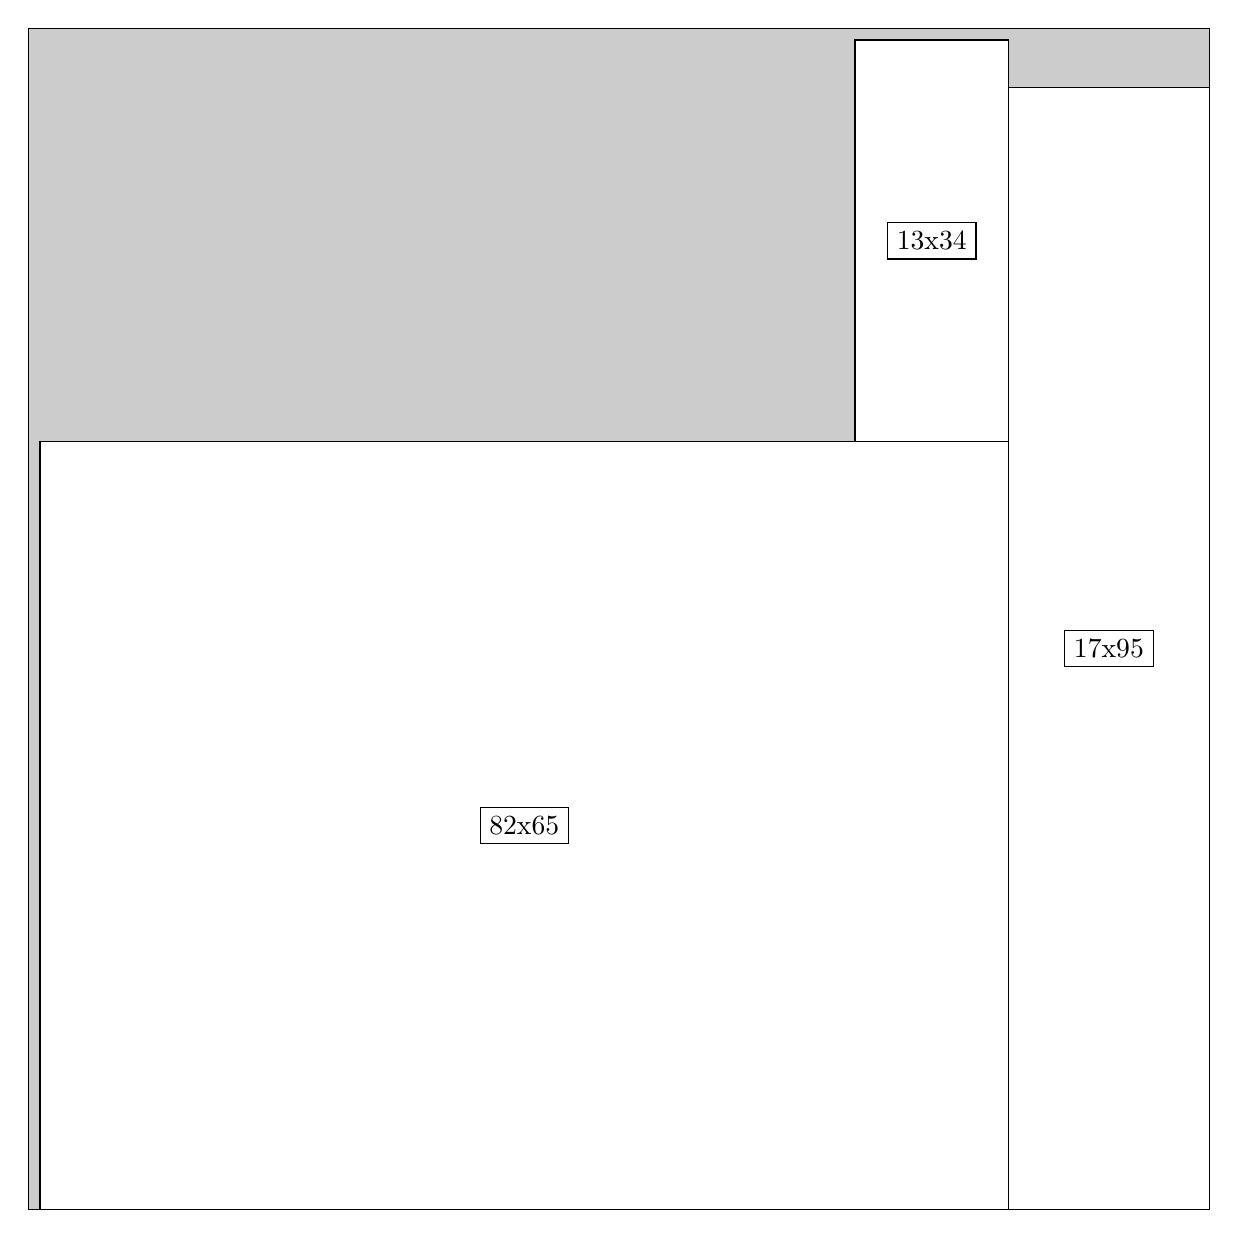
\begin{tikzpicture}[shorten >=1pt,scale=1.0,every node/.style={scale=1.0},->]
\tikzstyle{vertex}=[circle,fill=black!25,minimum size=14pt,inner sep=0pt]
\filldraw[fill=gray!40!white, draw=black] (0,0) rectangle (15.0,15.0);
\foreach \name/\x/\y/\w/\h in {17x95/12.45/0.0/2.55/14.25,82x65/0.15/0.0/12.299999999999999/9.75,13x34/10.5/9.75/1.95/5.1}
\filldraw[fill=white!40!white, draw=black] (\x,\y) rectangle node[draw] (\name) {\name} ++(\w,\h);
\end{tikzpicture}


w =17 , h =95 , x =83 , y =0 , v =1615
\par
w =82 , h =65 , x =1 , y =0 , v =5330
\par
w =13 , h =34 , x =70 , y =65 , v =442
\par
\newpage


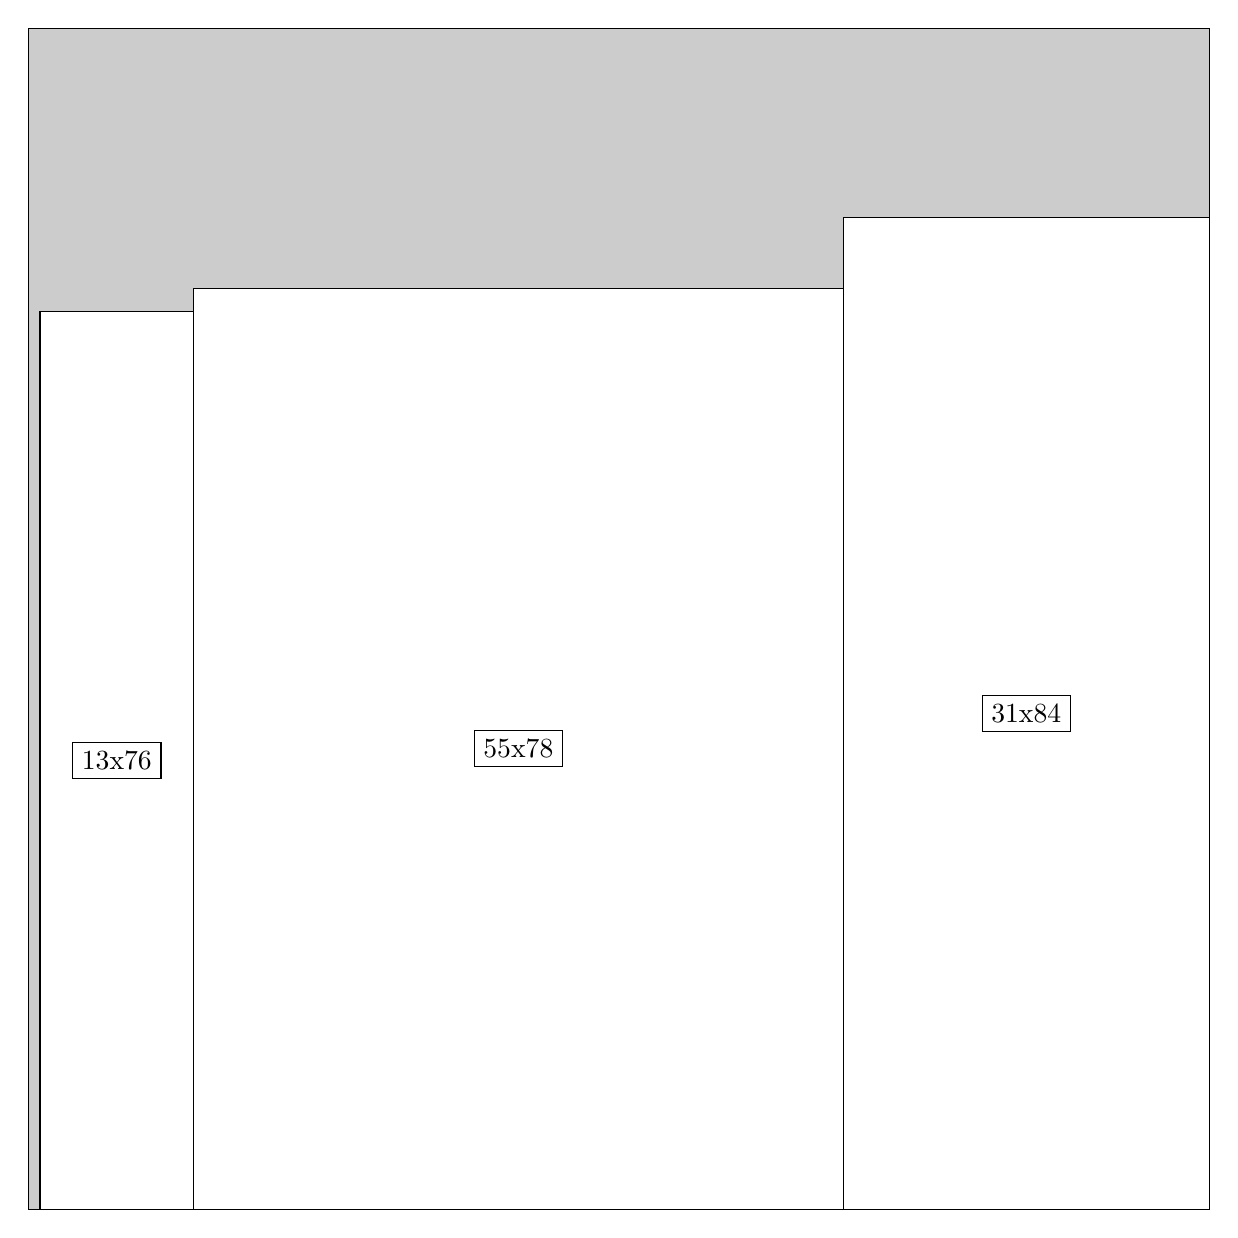
\begin{tikzpicture}[shorten >=1pt,scale=1.0,every node/.style={scale=1.0},->]
\tikzstyle{vertex}=[circle,fill=black!25,minimum size=14pt,inner sep=0pt]
\filldraw[fill=gray!40!white, draw=black] (0,0) rectangle (15.0,15.0);
\foreach \name/\x/\y/\w/\h in {31x84/10.35/0.0/4.6499999999999995/12.6,55x78/2.1/0.0/8.25/11.7,13x76/0.15/0.0/1.95/11.4}
\filldraw[fill=white!40!white, draw=black] (\x,\y) rectangle node[draw] (\name) {\name} ++(\w,\h);
\end{tikzpicture}


w =31 , h =84 , x =69 , y =0 , v =2604
\par
w =55 , h =78 , x =14 , y =0 , v =4290
\par
w =13 , h =76 , x =1 , y =0 , v =988
\par
\newpage


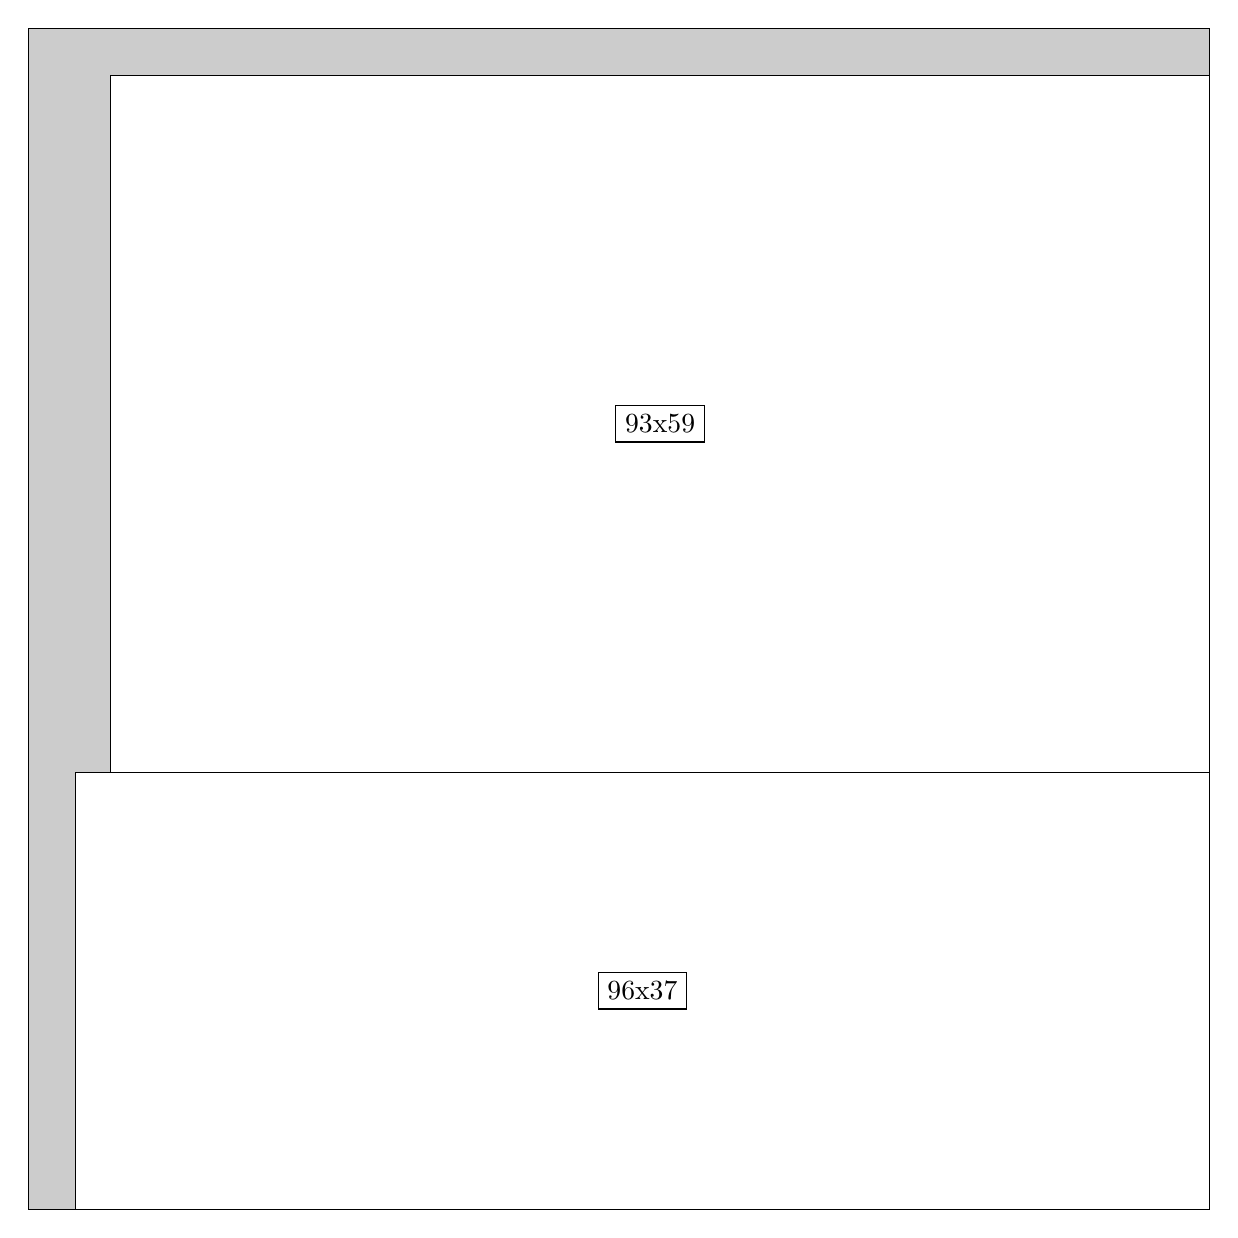
\begin{tikzpicture}[shorten >=1pt,scale=1.0,every node/.style={scale=1.0},->]
\tikzstyle{vertex}=[circle,fill=black!25,minimum size=14pt,inner sep=0pt]
\filldraw[fill=gray!40!white, draw=black] (0,0) rectangle (15.0,15.0);
\foreach \name/\x/\y/\w/\h in {96x37/0.6/0.0/14.399999999999999/5.55,93x59/1.05/5.55/13.95/8.85}
\filldraw[fill=white!40!white, draw=black] (\x,\y) rectangle node[draw] (\name) {\name} ++(\w,\h);
\end{tikzpicture}


w =96 , h =37 , x =4 , y =0 , v =3552
\par
w =93 , h =59 , x =7 , y =37 , v =5487
\par
\newpage


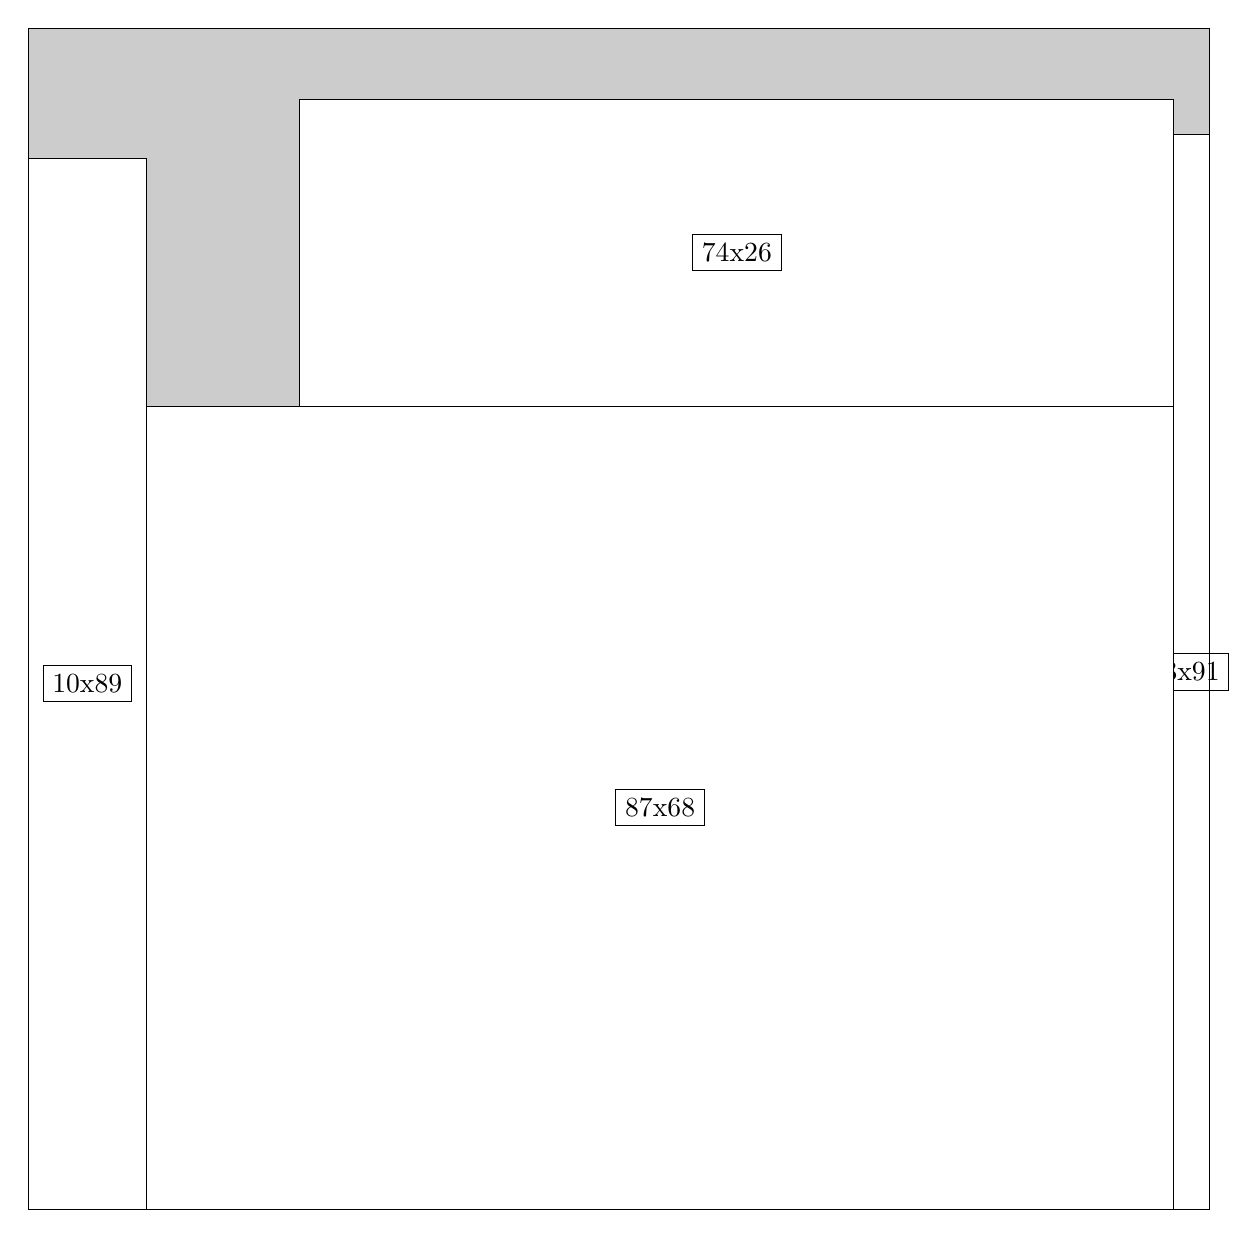
\begin{tikzpicture}[shorten >=1pt,scale=1.0,every node/.style={scale=1.0},->]
\tikzstyle{vertex}=[circle,fill=black!25,minimum size=14pt,inner sep=0pt]
\filldraw[fill=gray!40!white, draw=black] (0,0) rectangle (15.0,15.0);
\foreach \name/\x/\y/\w/\h in {3x91/14.549999999999999/0.0/0.44999999999999996/13.65,87x68/1.5/0.0/13.049999999999999/10.2,74x26/3.4499999999999997/10.2/11.1/3.9,10x89/0.0/0.0/1.5/13.35}
\filldraw[fill=white!40!white, draw=black] (\x,\y) rectangle node[draw] (\name) {\name} ++(\w,\h);
\end{tikzpicture}


w =3 , h =91 , x =97 , y =0 , v =273
\par
w =87 , h =68 , x =10 , y =0 , v =5916
\par
w =74 , h =26 , x =23 , y =68 , v =1924
\par
w =10 , h =89 , x =0 , y =0 , v =890
\par
\newpage


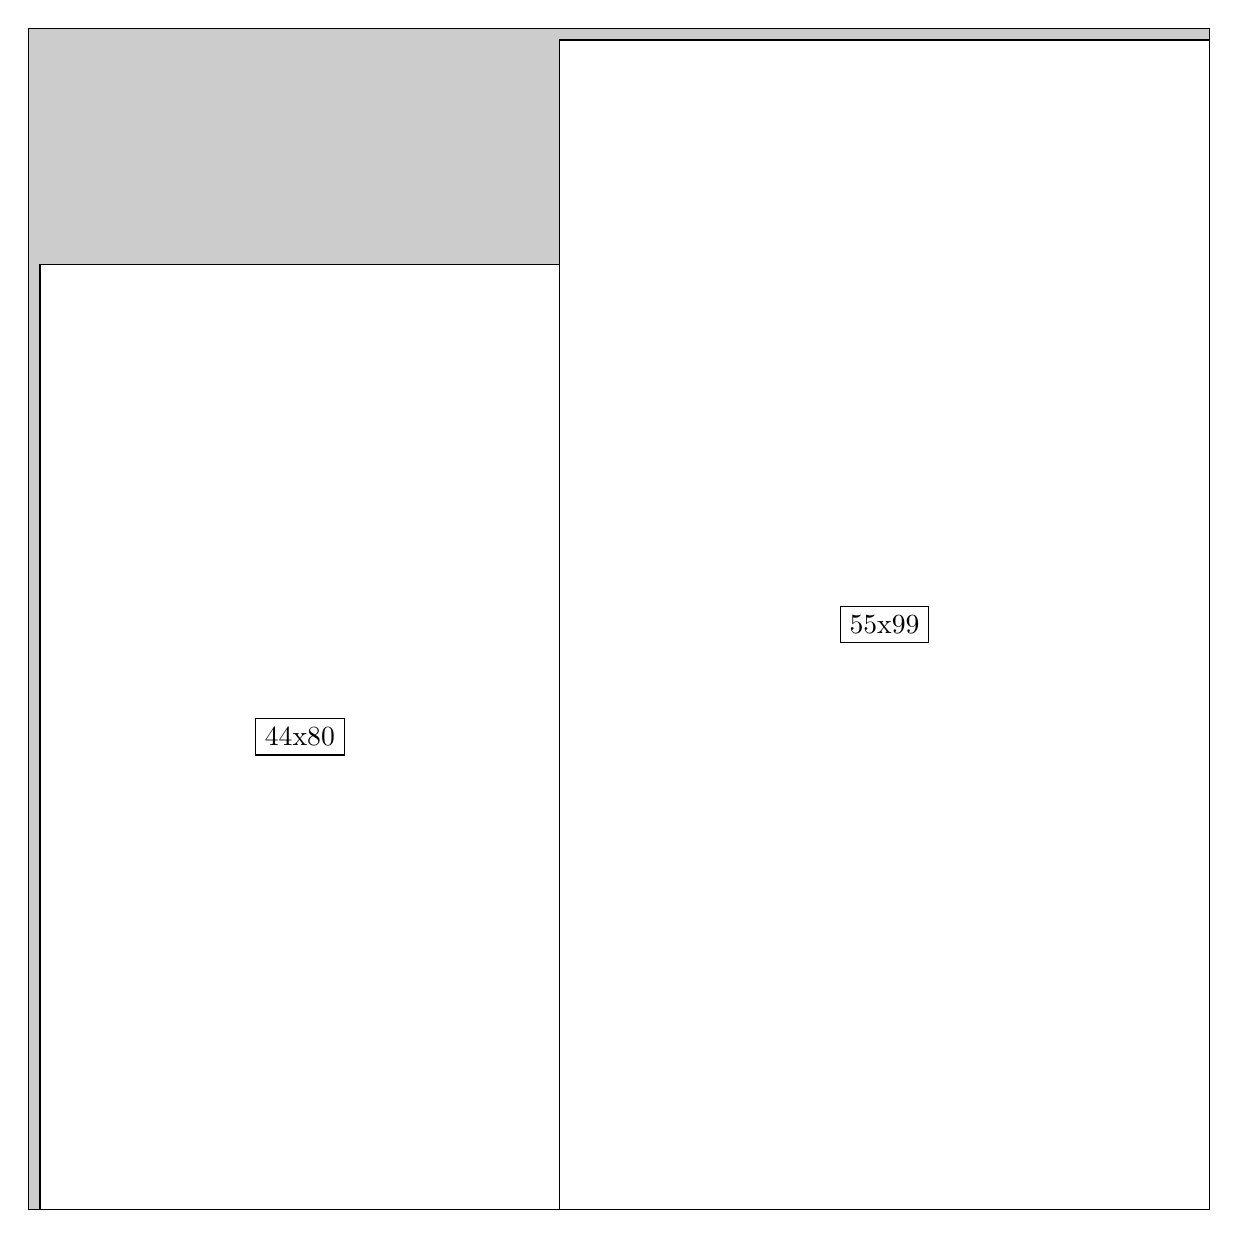
\begin{tikzpicture}[shorten >=1pt,scale=1.0,every node/.style={scale=1.0},->]
\tikzstyle{vertex}=[circle,fill=black!25,minimum size=14pt,inner sep=0pt]
\filldraw[fill=gray!40!white, draw=black] (0,0) rectangle (15.0,15.0);
\foreach \name/\x/\y/\w/\h in {55x99/6.75/0.0/8.25/14.85,44x80/0.15/0.0/6.6/12.0}
\filldraw[fill=white!40!white, draw=black] (\x,\y) rectangle node[draw] (\name) {\name} ++(\w,\h);
\end{tikzpicture}


w =55 , h =99 , x =45 , y =0 , v =5445
\par
w =44 , h =80 , x =1 , y =0 , v =3520
\par
\newpage


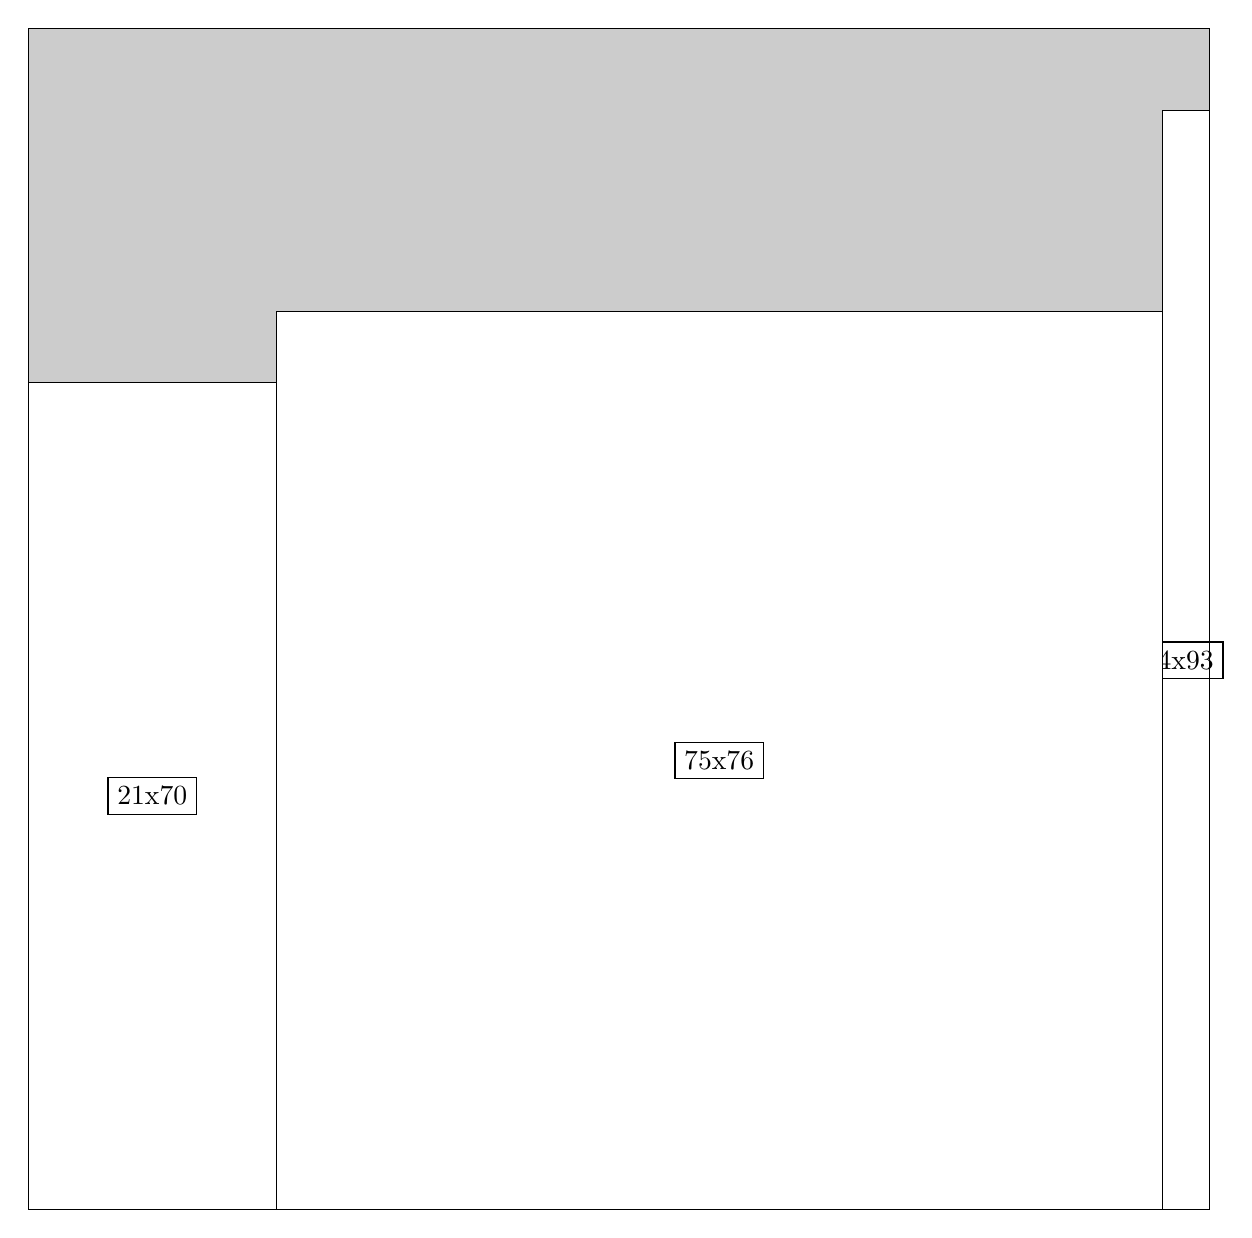
\begin{tikzpicture}[shorten >=1pt,scale=1.0,every node/.style={scale=1.0},->]
\tikzstyle{vertex}=[circle,fill=black!25,minimum size=14pt,inner sep=0pt]
\filldraw[fill=gray!40!white, draw=black] (0,0) rectangle (15.0,15.0);
\foreach \name/\x/\y/\w/\h in {4x93/14.399999999999999/0.0/0.6/13.95,75x76/3.15/0.0/11.25/11.4,21x70/0.0/0.0/3.15/10.5}
\filldraw[fill=white!40!white, draw=black] (\x,\y) rectangle node[draw] (\name) {\name} ++(\w,\h);
\end{tikzpicture}


w =4 , h =93 , x =96 , y =0 , v =372
\par
w =75 , h =76 , x =21 , y =0 , v =5700
\par
w =21 , h =70 , x =0 , y =0 , v =1470
\par
\newpage


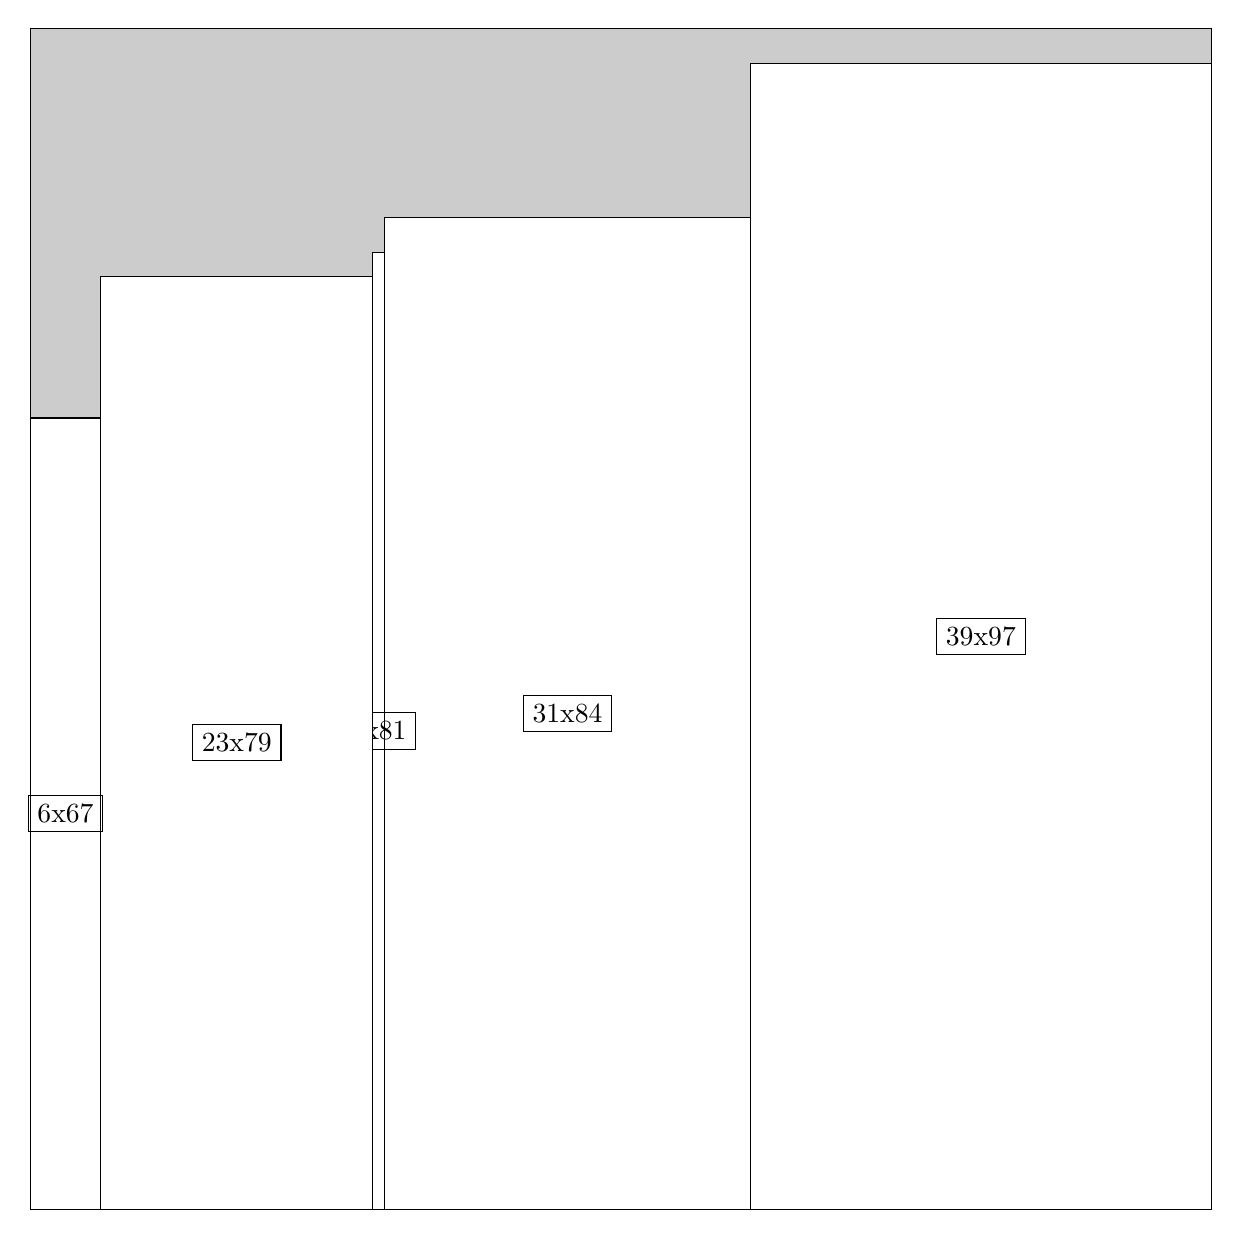
\begin{tikzpicture}[shorten >=1pt,scale=1.0,every node/.style={scale=1.0},->]
\tikzstyle{vertex}=[circle,fill=black!25,minimum size=14pt,inner sep=0pt]
\filldraw[fill=gray!40!white, draw=black] (0,0) rectangle (15.0,15.0);
\foreach \name/\x/\y/\w/\h in {39x97/9.15/0.0/5.85/14.549999999999999,31x84/4.5/0.0/4.6499999999999995/12.6,1x81/4.35/0.0/0.15/12.15,23x79/0.8999999999999999/0.0/3.4499999999999997/11.85,6x67/0.0/0.0/0.8999999999999999/10.049999999999999}
\filldraw[fill=white!40!white, draw=black] (\x,\y) rectangle node[draw] (\name) {\name} ++(\w,\h);
\end{tikzpicture}


w =39 , h =97 , x =61 , y =0 , v =3783
\par
w =31 , h =84 , x =30 , y =0 , v =2604
\par
w =1 , h =81 , x =29 , y =0 , v =81
\par
w =23 , h =79 , x =6 , y =0 , v =1817
\par
w =6 , h =67 , x =0 , y =0 , v =402
\par
\newpage


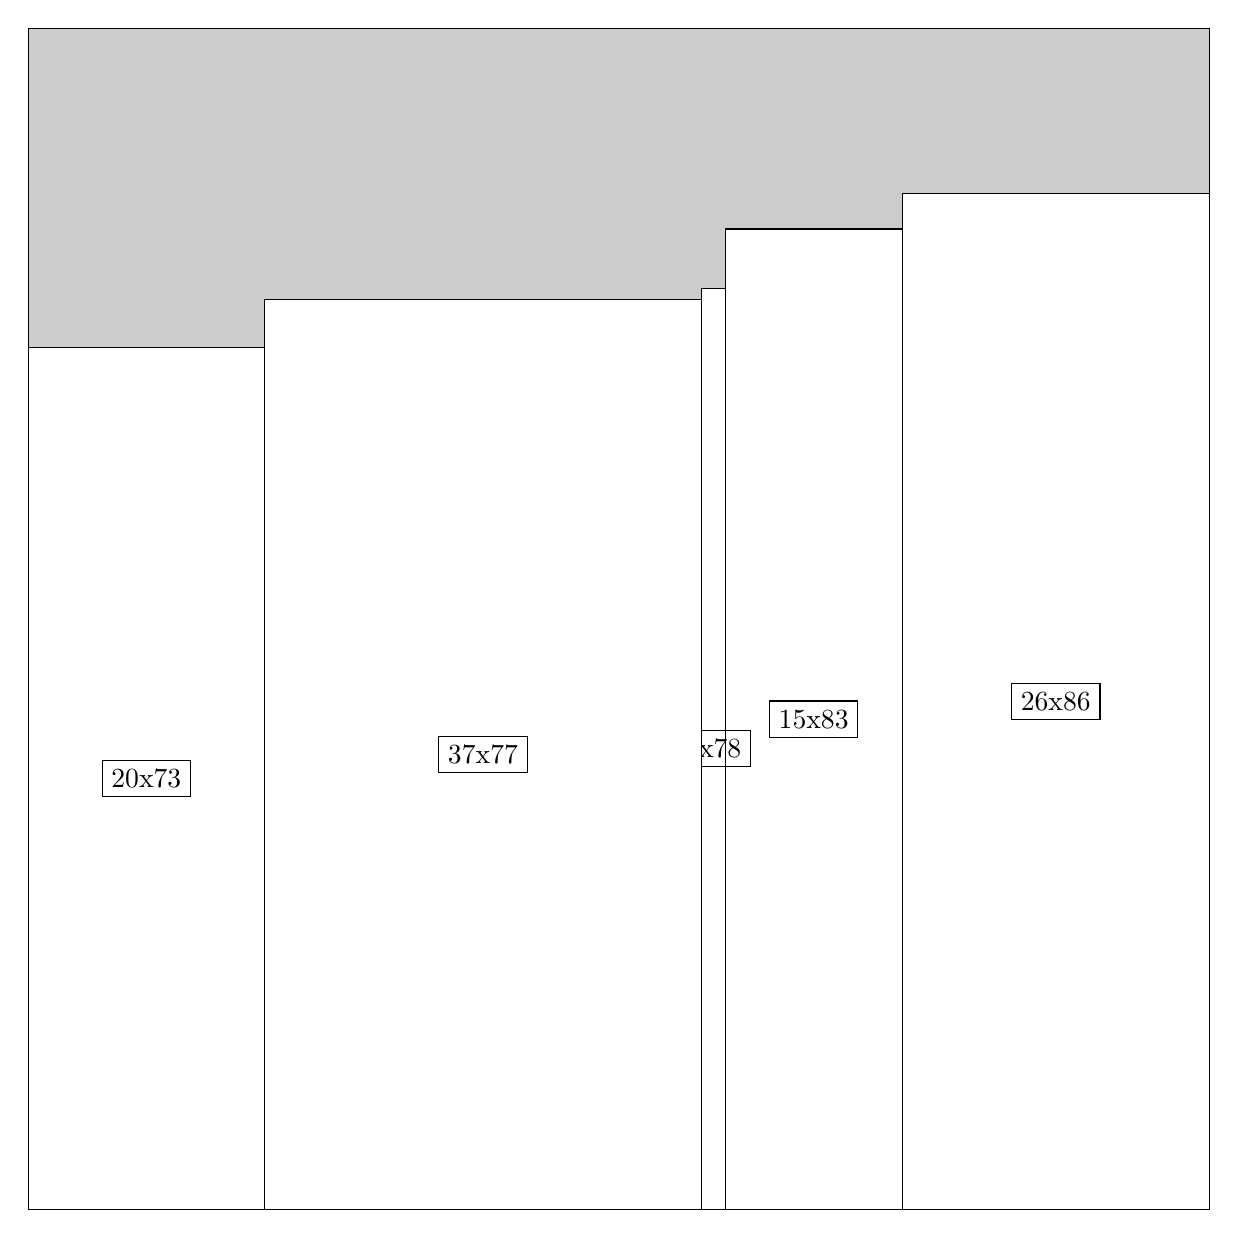
\begin{tikzpicture}[shorten >=1pt,scale=1.0,every node/.style={scale=1.0},->]
\tikzstyle{vertex}=[circle,fill=black!25,minimum size=14pt,inner sep=0pt]
\filldraw[fill=gray!40!white, draw=black] (0,0) rectangle (15.0,15.0);
\foreach \name/\x/\y/\w/\h in {26x86/11.1/0.0/3.9/12.9,15x83/8.85/0.0/2.25/12.45,2x78/8.549999999999999/0.0/0.3/11.7,37x77/3.0/0.0/5.55/11.549999999999999,20x73/0.0/0.0/3.0/10.95}
\filldraw[fill=white!40!white, draw=black] (\x,\y) rectangle node[draw] (\name) {\name} ++(\w,\h);
\end{tikzpicture}


w =26 , h =86 , x =74 , y =0 , v =2236
\par
w =15 , h =83 , x =59 , y =0 , v =1245
\par
w =2 , h =78 , x =57 , y =0 , v =156
\par
w =37 , h =77 , x =20 , y =0 , v =2849
\par
w =20 , h =73 , x =0 , y =0 , v =1460
\par
\newpage


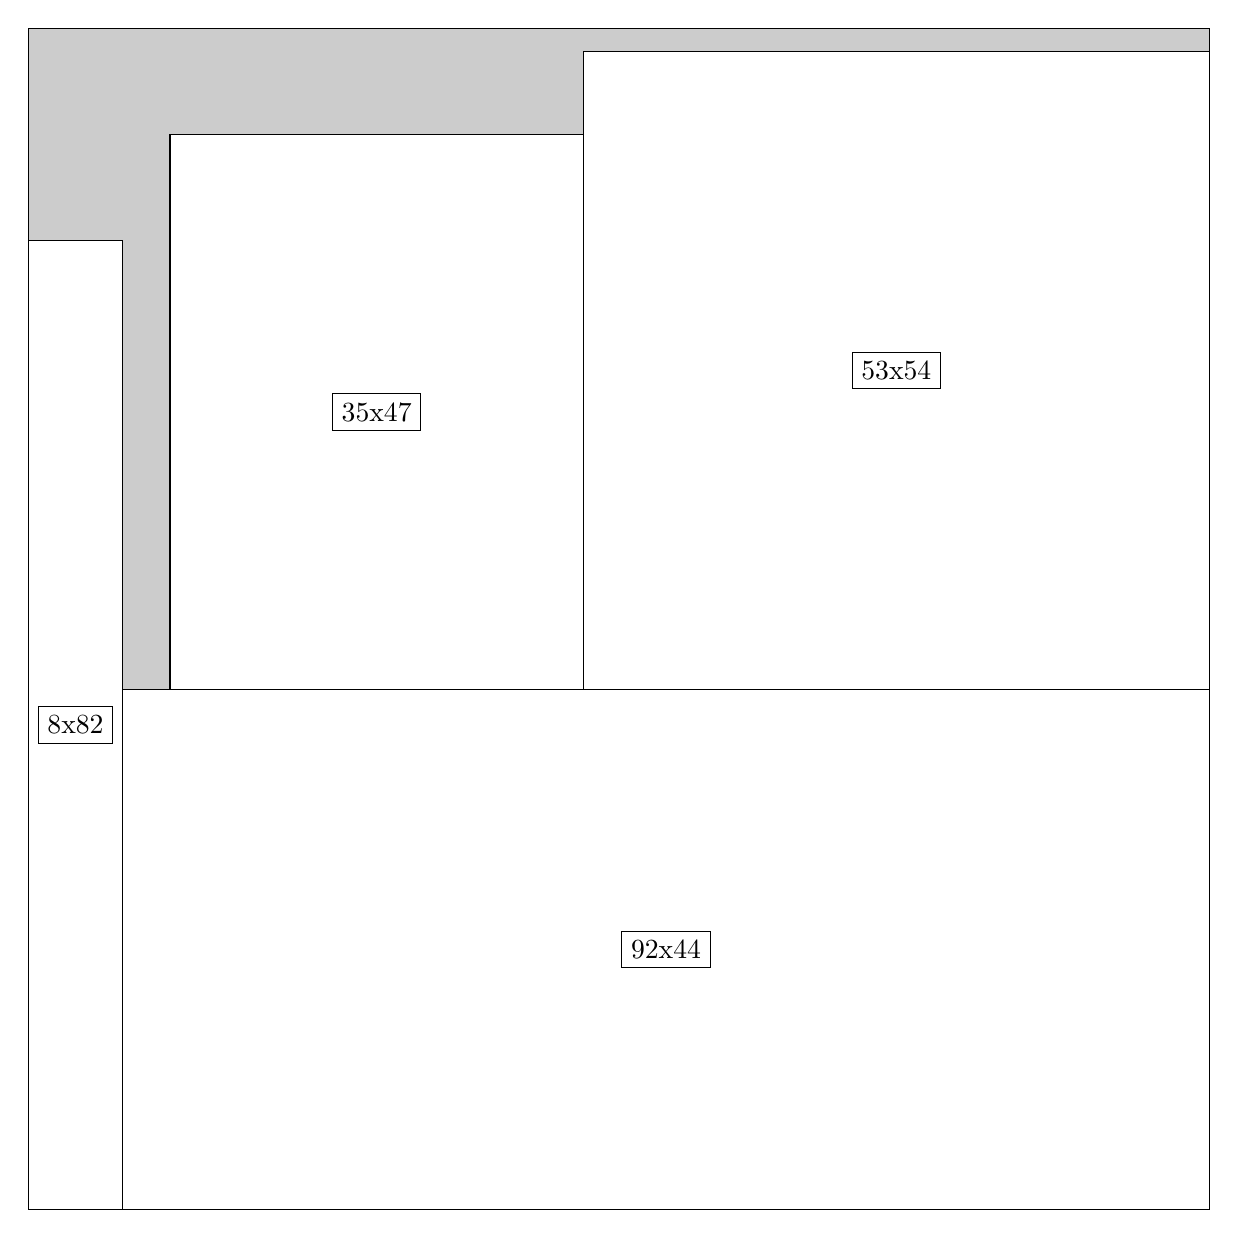
\begin{tikzpicture}[shorten >=1pt,scale=1.0,every node/.style={scale=1.0},->]
\tikzstyle{vertex}=[circle,fill=black!25,minimum size=14pt,inner sep=0pt]
\filldraw[fill=gray!40!white, draw=black] (0,0) rectangle (15.0,15.0);
\foreach \name/\x/\y/\w/\h in {92x44/1.2/0.0/13.799999999999999/6.6,53x54/7.05/6.6/7.949999999999999/8.1,35x47/1.7999999999999998/6.6/5.25/7.05,8x82/0.0/0.0/1.2/12.299999999999999}
\filldraw[fill=white!40!white, draw=black] (\x,\y) rectangle node[draw] (\name) {\name} ++(\w,\h);
\end{tikzpicture}


w =92 , h =44 , x =8 , y =0 , v =4048
\par
w =53 , h =54 , x =47 , y =44 , v =2862
\par
w =35 , h =47 , x =12 , y =44 , v =1645
\par
w =8 , h =82 , x =0 , y =0 , v =656
\par
\newpage


\end{document}